% das Papierformat zuerst
\documentclass[a4paper, 11pt]{article}
% deutsche Silbentrennung
\usepackage[ngerman]{babel}
% wegen deutschen Umlauten
\usepackage[utf8]{inputenc}
% andere pdfs einbinden
\usepackage{pdfpages}
% um bilder einzubinden
\usepackage{graphicx}
% fuer source code listings
\usepackage{listings}
% seitenränder
\usepackage[left=3cm,right=3cm,top=2cm,bottom=2cm]{geometry}
% um hyperlinks einfügen zu können
\usepackage{hyperref}

\begin{document}

% Den Titel festlegen
\title{Elektrotechnik Laborprotokoll\\Praktikumsaufgabe 1}

% Zwei Autoren
\author{Max Mustermann (Matrikelnummer: 123456789) \and 
        Hans Hase (Matrikelnummer: 987654321)}

% Erstelle die Titelseite
\maketitle 
\newpage % Neue Seite

% Erstelle das Inhaltsverzeichnis
\tableofcontents
\newpage % Wir wollen das Inhaltsverzeichnis auf einer eigenen Seite

%%%%%%%%%%%%%%%%%%%%%%%%%%%%%%%%%%%%%%%%%
% Das erste Kapitel
%%%%%%%%%%%%%%%%%%%%%%%%%%%%%%%%%%%%%%%%%
\section{Einleitung}
Hier steht eine allgemeine Beschreibung der Praktikumsaufgabe
\newpage

%%%%%%%%%%%%%%%%%%%%%%%%%%%%%%%%%%%%%%%%%
% Das erste Kapitel
%%%%%%%%%%%%%%%%%%%%%%%%%%%%%%%%%%%%%%%%%
\section{Durchführung}
Hier steht das zweite Kapitel

% Ein Unterkapitel
\subsection{Messung}
Dies ist ein Unterkapitel
\newpage

\subsection{Berechnungen}

Hier ist ein einfacher Ausdruck: $\sin(\frac{30 \pi}{180})^{2} + \cos(\frac{30 \pi}{180})^{2} = 1$
\\
\\
Hier wird es ein bisschen komplexer: 
\begin{eqnarray}\nonumber
\xi_1(t) + \xi_2(t) &=& \xi_0\,\left(\sin(\omega_1 t)+\sin(\omega_2 t)\right) \\ \nonumber
    &=& 2\xi_0\, \underbrace{\sin\left(\frac{(\omega_1+\omega_2)\, t}{2}\right)}_{\mbox{\scriptsize Schwingung mit $\frac{\omega_1+\omega_2}{2}$}}\cdot \underbrace{\cos\left(\frac{(\omega_1-\omega_2)\, t}{2}\right)}_{\mbox{\scriptsize Modulation mit $\frac{\omega_1-\omega_2}{2}$}}
\end{eqnarray}

\subsection*{Tabellen} % Dieses Kapitel wird NICHT im Inhaltsverzeichnis angezeigt, siehe Sternen ;)
\begin{center}
\begin{table}[h] % genau hier einfügen
\begin{tabular}{ l | c || r } % ausrichtung definieren
\hline % horizontale Linie
\textbf{Funktion} & \textbf{Bedeutung} & \textbf{Definitionsbereich} \\ \hline\hline
$acos(x)$  & arcos von x & 0 bis $\pi$ \\ \hline
$asin(x)$  & arcsin von x & $\frac{-\pi}{2}$ bis $\frac{\pi}{2}$ \\ \hline
\end{tabular}
\caption{Funktionsübersicht}
\end{table}
\end{center}

\subsection{Bilder}
\begin{figure}[h]
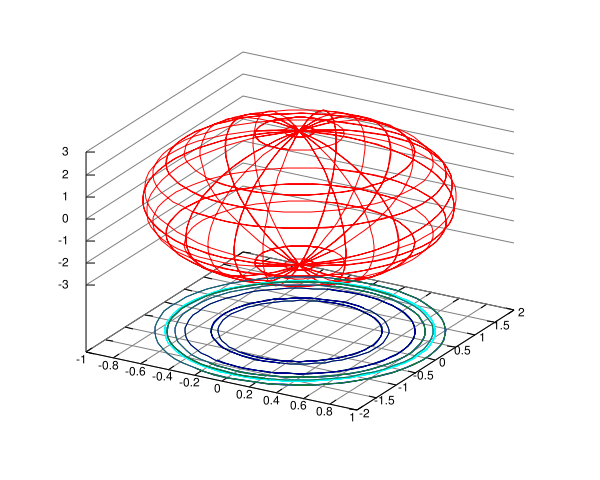
\includegraphics[scale=0.5]{gnuplot.png} 
\caption{Ein Bild}
\end{figure}

%
% Ende, jetzt noch der Anhang
%
\newpage
\listoftables  % Tabellenverzeichnis erstellen
\listoffigures % Abbildungsverzeichnis erstellen
\end{document}
